%% =============================================================
%%  Guitar Chord Reference --- Comprehensive Visual Guide
%%  Standard Tuning: E A D G B e
%% =============================================================
\documentclass[a4paper,10pt]{article}

\usepackage[top=2.2cm,bottom=2.4cm,left=1.7cm,right=1.7cm]{geometry}
\usepackage{tikz}
\usepackage{xcolor}
\usepackage[T1]{fontenc}
\usepackage[utf8]{inputenc}
\usepackage{titlesec}
\usepackage{etoolbox}
\usepackage{fancyhdr}
\usepackage{mdframed}
\usepackage{array}
\usepackage{enumitem}
\usepackage{booktabs}
\usepackage{graphicx}
\usepackage{colortbl}
\usepackage{longtable}
% Les portées sont engendrées par outils/generer.py depuis les doigtés
% ci-dessous : elles ne peuvent donc pas contredire leur diagramme.
\graphicspath{{gravures/}}

\hfuzz=10pt

% ---- Colours -------------------------------------------------------
\definecolor{navy}{RGB}{18,50,105}
\definecolor{lightnavy}{RGB}{235,241,255}
\definecolor{mygray}{RGB}{110,110,110}
\definecolor{rowA}{RGB}{245,248,255}
\definecolor{rowB}{RGB}{255,255,255}

% ---- Header / footer -----------------------------------------------
\pagestyle{fancy}
\fancyhf{}
\renewcommand{\headrulewidth}{0.4pt}
\renewcommand{\footrulewidth}{0.4pt}
\fancyhead[L]{\small\bfseries\textcolor{navy}{Guitar Chord Reference}}
\fancyhead[R]{\small\textcolor{mygray}{\thepage}}
\fancyfoot[C]{\small\textcolor{mygray}{Standard Tuning (low to high):
  \textbf{E\;--\;A\;--\;D\;--\;G\;--\;B\;--\;e}}}

% ---- Section headings ----------------------------------------------
\newcommand{\navysect}[1]{%
  \colorbox{navy}{%
    \parbox[c][15pt]{\dimexpr\linewidth-2\fboxsep\relax}{%
      \color{white}\hspace{6pt}\bfseries\normalsize #1}}%
}
\titleformat{\section}[block]{\normalfont}{}{0pt}{\navysect}
\titlespacing*{\section}{0pt}{14pt}{8pt}

\titleformat{\subsection}
  {\normalfont\small\bfseries\color{navy}}{}{0pt}{}
\titlespacing*{\subsection}{0pt}{8pt}{4pt}

% ====================================================================
%  CHORD DIAGRAM MACRO
% ====================================================================
\def\MUTE{x}
\def\OPEN{o}

\newcommand{\chord}[5]{%
  \begin{tikzpicture}[x=0.40cm, y=0.40cm, baseline=(cname.base)]
    \node[font=\small\bfseries, color=navy, anchor=base]
      (cname) at (3.5, 0.78) {#1};
    \pgfmathtruncatemacro{\SF}{#2}%
    \ifnum\SF=1
      \draw[line width=3pt, color=black] (0.72,-0.5) -- (6.28,-0.5);
    \else
      \node[font=\scriptsize\bfseries, color=navy, anchor=east, overlay]
        at (0.45,-1.0) {\SF};
    \fi
    \foreach \s in {1,...,6}{\draw[color=black!50, thin] (\s,-0.5) -- (\s,-4.5);}
    \foreach \f in {0,...,4}{\draw[color=black!50, thin] (1,{-0.5-\f}) -- (6,{-0.5-\f});}
    \ifblank{#3}{}{%
      \foreach \SI/\TI in {#3}{%
        \ifx\TI\MUTE
          \node[font=\normalsize, color=black!65] at (\SI, 0.08){$\times$};%
        \else
          \node[font=\normalsize, color=navy!80] at (\SI, 0.08){$\circ$};%
        \fi}}%
    \ifblank{#4}{}{%
      \foreach \LO/\HI/\BF in {#4}{%
        \draw[line width=5pt, color=navy, line cap=round]
          (\LO,{-\BF}) -- (\HI,{-\BF});}}%
    \ifblank{#5}{}{%
      \foreach \SD/\FD in {#5}{%
        \fill[navy] (\SD,{-\FD}) circle (0.125cm);}}%
  \end{tikzpicture}%
}

% Chord + staff wrapper
\newcommand{\cw}[2]{%
  \parbox[b]{2.75cm}{\centering
    #2\newline
    \includegraphics[width=1.90cm]{#1_t.cropped}%
  }%
}

% Centred row of up to 6 chord+staff cells
\newenvironment{chordrow}{%
  \begin{center}\setlength{\tabcolsep}{0.20em}%
  \begin{tabular}{cccccc}%
}{%
  \end{tabular}\end{center}%
}

% ====================================================================
\begin{document}
\thispagestyle{empty}

% ---- Title block ---------------------------------------------------
\begin{tikzpicture}[remember picture, overlay]
  \fill[navy] (current page.north west)
    rectangle ([yshift=-5.1cm]current page.north east);
  \node[anchor=north west, white,
        font=\fontsize{28}{32}\selectfont\bfseries]
    at ([xshift=1.7cm, yshift=-1.0cm]current page.north west)
    {Guitar Chord Reference};
  \node[anchor=north west, white!80!navy, font=\large]
    at ([xshift=1.7cm, yshift=-2.15cm]current page.north west)
    {A Comprehensive Visual Guide
     \quad Standard Tuning: E -- A -- D -- G -- B -- e};
  \node[anchor=north west, white!60!navy, font=\normalsize]
    at ([xshift=1.7cm, yshift=-3.0cm]current page.north west)
    {Theory (A -- G) $\cdot$ Open chords $\cdot$ Barre chords $\cdot$
     7ths $\cdot$ Sus $\cdot$ Power $\cdot$ Add9 $\cdot$ Aug $\cdot$ Dim};
\end{tikzpicture}

\vspace*{5.4cm}

% ---- Introduction --------------------------------------------------
\noindent
This guide is a self-contained reference for guitarists at any level,
from the first open chord to complex jazz voicings.
It is organised in three parts.

\medskip
\noindent
The \textbf{theory chapter}
(pages~\pageref{deb-theorie}--\pageref{fin-theorie}) explains how chord
symbols work: what the letters and suffixes mean, and how every chord
type is built from a scale.
Each of the seven natural roots (A through G) gets its own table,
with close-position staff notation in the treble-8 clef standard
to guitar.

\medskip
\noindent
The \textbf{chord diagram sections}
(pages~\pageref{deb-diagrammes}--\pageref{fin-diagrammes}) provide
fingering diagrams and staff notation for more than sixty voicings
in standard tuning: open major and minor chords, dominant and major
seventh chords, suspended, power, barre, add9, augmented and
diminished chords, and the diatonic chords of C major, with the Roman
numerals that transpose any progression to a new key.

\medskip
\noindent
The \textbf{practical sections}
(pages~\pageref{deb-pratique}--\pageref{fin-pratique}) bridge theory and
playing: a primer on strumming patterns and rhythm notation, four
graded songs (beginner to intermediate) with chord grids and
picking patterns, and a set of technique tips for cleaner fretting,
smoother chord changes and better barre chords.

\medskip
\noindent
All diagrams assume \textbf{standard tuning}
(low to high: E -- A -- D -- G -- B -- e).
Staff notation uses the \textbf{treble-8 clef} (sounds one octave
below written), which is the international standard for guitar.

\clearpage
\thispagestyle{empty}
{\small\tableofcontents}
\clearpage

% ====================================================================
\section{How to Read Chord Diagrams}

\begin{mdframed}[backgroundcolor=lightnavy, linecolor=navy,
                 linewidth=0.8pt, innerleftmargin=10pt,
                 innerrightmargin=10pt, innertopmargin=8pt,
                 innerbottommargin=8pt]
\begin{minipage}[t]{0.55\linewidth}\small
Each diagram shows the guitar neck as seen from the front.
Strings are \textbf{vertical} (low E at left, high e at right);
frets are \textbf{horizontal}.
\begin{itemize}[nosep, leftmargin=1.3em]
  \item \textbf{Thick top bar} = the nut (open-position chords)
  \item \textbf{Number at left} = starting fret (barre chords)
  \item \textbf{Filled circles} = press here with your fingertip
  \item \textbf{Thick round bar} = barre (one finger across multiple strings)
  \item {\large$\circ$} above string = play it \emph{open} (unfretted)
  \item {\large$\times$} above string = mute / do not play
\end{itemize}
\smallskip
The \textbf{staff notation} below each diagram uses the \textit{treble-8} clef
--- standard for guitar. Notes are written an octave higher than they sound;
the ``8'' below the clef is a reminder to read them down one octave.
Finger numbers: \textbf{1}=index\ \textbf{2}=middle\
\textbf{3}=ring\ \textbf{4}=pinky.
\end{minipage}%
\hfill
\begin{minipage}[t]{0.38\linewidth}\centering\small
\textit{Example: C major (x32010)}\\[0.4em]
\cw{C}{\chord{C major}{1}{1/x,4/o,6/o}{}{2/3,3/2,5/1}}
\end{minipage}
\end{mdframed}

% ====================================================================
\section{Chord Theory: Chord Families A through G}
\label{deb-theorie}

\noindent
A chord symbol has two parts: a \textbf{root} (the letter name)
and a \textbf{quality descriptor} that specifies the interval structure.
The tables below show every chord type for each of the seven natural roots
\textbf{A, B, C, D, E, F, G}.
Formulas use \emph{scale-degree numbers} with accidentals
($\flat$ = lower by 1 semitone, $\sharp$ = raise by 1 semitone).
The \textbf{Staff} column shows the chord in close position using the
treble-8 clef; guitar diagrams on later pages show practical voicings
on the fretboard.

\smallskip

%% Produit par outils/generer.py — ne pas modifier à la main.

\subsection*{The A Family}
\noindent\textbf{Key signature:} three sharps: F$\sharp$, C$\sharp$, G$\sharp$.\smallskip

\begin{center}
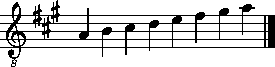
\includegraphics[height=1.15cm]{scale-A.cropped}\\[2pt]
{\small\color{mygray}\textbf{1} A\quad \textbf{2} B\quad \textbf{3} C$\sharp$\quad \textbf{4} D\quad \textbf{5} E\quad \textbf{6} F$\sharp$\quad \textbf{7} G$\sharp$\quad \textbf{8} A}
\end{center}

\begin{longtable}{@{}l l l c >{\raggedright\arraybackslash}p{4.4cm}@{}}
\toprule
\textbf{Symbol} & \textbf{Full name} & \textbf{Formula} & \textbf{Staff} & \textbf{Colour / use} \\
\midrule\endhead
\rowcolor{rowA}
\textbf{A} & A major & 1 -- 3 -- 5 & 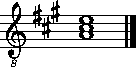
\includegraphics[height=1.15cm]{th-Amaj.cropped} & Bright, stable. \\
\rowcolor{rowB}
\textbf{Am} & A minor & 1 -- $\flat$3 -- 5 & 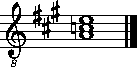
\includegraphics[height=1.15cm]{th-Am.cropped} & Dark. Lower the 3rd: C$\sharp$ $\to$ C. \\
\rowcolor{rowA}
\textbf{A5} & A power chord & 1 -- 5 & 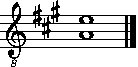
\includegraphics[height=1.15cm]{th-A5.cropped} & Raw, neutral. No 3rd. \\
\rowcolor{rowB}
\textbf{Asus2} & A sus. 2nd & 1 -- 2 -- 5 & 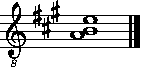
\includegraphics[height=1.15cm]{th-Asus2.cropped} & Open. Replace 3rd with 2nd (B). \\
\rowcolor{rowA}
\textbf{Asus4} & A sus. 4th & 1 -- 4 -- 5 & 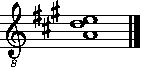
\includegraphics[height=1.15cm]{th-Asus4.cropped} & Tense. Replace 3rd with 4th (D). \\
\rowcolor{rowB}
\textbf{A6} & A major sixth & 1 -- 3 -- 5 -- 6 & 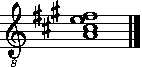
\includegraphics[height=1.15cm]{th-A6.cropped} & Sweet, vintage. Add 6th (F$\sharp$). \\
\rowcolor{rowA}
\textbf{Aadd9} & A add nine & 1 -- 3 -- 5 -- 9 & 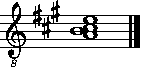
\includegraphics[height=1.15cm]{th-Aadd9.cropped} & Colourful. Add 2nd/9th (B), no 7th. \\
\rowcolor{rowB}
\textbf{A7} & A dominant 7th & 1 -- 3 -- 5 -- $\flat$7 & 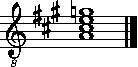
\includegraphics[height=1.15cm]{th-A7.cropped} & Bluesy. Lower 7th: G$\sharp$ $\to$ G. \\
\rowcolor{rowA}
\textbf{Amaj7} & A major 7th & 1 -- 3 -- 5 -- 7 & 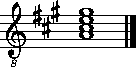
\includegraphics[height=1.15cm]{th-Amaj7.cropped} & Dreamy, jazzy. Keep natural 7th (G$\sharp$). \\
\rowcolor{rowB}
\textbf{Am7} & A minor 7th & 1 -- $\flat$3 -- 5 -- $\flat$7 & 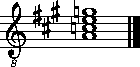
\includegraphics[height=1.15cm]{th-Am7.cropped} & Mellow, soulful. Lower 3rd and 7th. \\
\rowcolor{rowA}
\textbf{Aaug} & A augmented & 1 -- 3 -- $\sharp$5 & 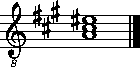
\includegraphics[height=1.15cm]{th-Aaug.cropped} & Eerie. Raise the 5th by 1 semitone. \\
\rowcolor{rowB}
\textbf{Adim} & A diminished & 1 -- $\flat$3 -- $\flat$5 & 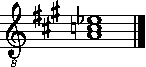
\includegraphics[height=1.15cm]{th-Adim.cropped} & Very tense. Lower 3rd and 5th. \\
\rowcolor{rowA}
\textbf{Adim7} & A dim. 7th & 1 -- $\flat$3 -- $\flat$5 -- $\flat\flat$7 & 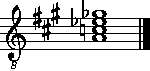
\includegraphics[height=1.15cm]{th-Adim7.cropped} & Max. tense. All minor 3rds. \\
\rowcolor{rowB}
\textbf{Am7$\flat$5} & A half-dim. & 1 -- $\flat$3 -- $\flat$5 -- $\flat$7 & 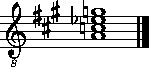
\includegraphics[height=1.15cm]{th-Am7b5.cropped} & Tense, jazzy (also: A\o). \\
\bottomrule
\end{longtable}

\subsection*{The B Family}
\noindent\textbf{Key signature:} five sharps: F$\sharp$, C$\sharp$, G$\sharp$, D$\sharp$, A$\sharp$.\smallskip

\begin{center}
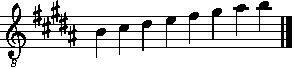
\includegraphics[height=1.15cm]{scale-B.cropped}\\[2pt]
{\small\color{mygray}\textbf{1} B\quad \textbf{2} C$\sharp$\quad \textbf{3} D$\sharp$\quad \textbf{4} E\quad \textbf{5} F$\sharp$\quad \textbf{6} G$\sharp$\quad \textbf{7} A$\sharp$\quad \textbf{8} B}
\end{center}

\begin{longtable}{@{}l l l c >{\raggedright\arraybackslash}p{4.4cm}@{}}
\toprule
\textbf{Symbol} & \textbf{Full name} & \textbf{Formula} & \textbf{Staff} & \textbf{Colour / use} \\
\midrule\endhead
\rowcolor{rowA}
\textbf{B} & B major & 1 -- 3 -- 5 & 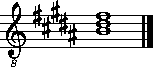
\includegraphics[height=1.15cm]{th-Bmaj.cropped} & Bright, stable. \\
\rowcolor{rowB}
\textbf{Bm} & B minor & 1 -- $\flat$3 -- 5 & 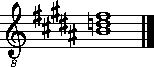
\includegraphics[height=1.15cm]{th-Bm.cropped} & Dark. Lower the 3rd: D$\sharp$ $\to$ D. \\
\rowcolor{rowA}
\textbf{B5} & B power chord & 1 -- 5 & 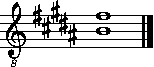
\includegraphics[height=1.15cm]{th-B5.cropped} & Raw, neutral. No 3rd. \\
\rowcolor{rowB}
\textbf{Bsus2} & B sus. 2nd & 1 -- 2 -- 5 & 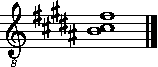
\includegraphics[height=1.15cm]{th-Bsus2.cropped} & Open. Replace 3rd with 2nd (C$\sharp$). \\
\rowcolor{rowA}
\textbf{Bsus4} & B sus. 4th & 1 -- 4 -- 5 & 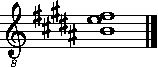
\includegraphics[height=1.15cm]{th-Bsus4.cropped} & Tense. Replace 3rd with 4th (E). \\
\rowcolor{rowB}
\textbf{B6} & B major sixth & 1 -- 3 -- 5 -- 6 & 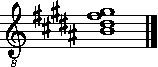
\includegraphics[height=1.15cm]{th-B6.cropped} & Sweet, vintage. Add 6th (G$\sharp$). \\
\rowcolor{rowA}
\textbf{Badd9} & B add nine & 1 -- 3 -- 5 -- 9 & 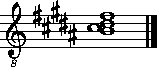
\includegraphics[height=1.15cm]{th-Badd9.cropped} & Colourful. Add 2nd/9th (C$\sharp$), no 7th. \\
\rowcolor{rowB}
\textbf{B7} & B dominant 7th & 1 -- 3 -- 5 -- $\flat$7 & 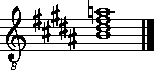
\includegraphics[height=1.15cm]{th-B7.cropped} & Bluesy. Lower 7th: A$\sharp$ $\to$ A. \\
\rowcolor{rowA}
\textbf{Bmaj7} & B major 7th & 1 -- 3 -- 5 -- 7 & 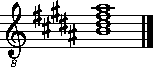
\includegraphics[height=1.15cm]{th-Bmaj7.cropped} & Dreamy, jazzy. Keep natural 7th (A$\sharp$). \\
\rowcolor{rowB}
\textbf{Bm7} & B minor 7th & 1 -- $\flat$3 -- 5 -- $\flat$7 & 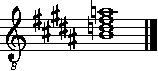
\includegraphics[height=1.15cm]{th-Bm7.cropped} & Mellow, soulful. Lower 3rd and 7th. \\
\rowcolor{rowA}
\textbf{Baug} & B augmented & 1 -- 3 -- $\sharp$5 & 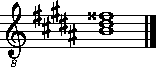
\includegraphics[height=1.15cm]{th-Baug.cropped} & Eerie. Raise the 5th by 1 semitone. \\
\rowcolor{rowB}
\textbf{Bdim} & B diminished & 1 -- $\flat$3 -- $\flat$5 & 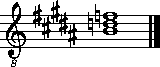
\includegraphics[height=1.15cm]{th-Bdim.cropped} & Very tense. Lower 3rd and 5th. \\
\rowcolor{rowA}
\textbf{Bdim7} & B dim. 7th & 1 -- $\flat$3 -- $\flat$5 -- $\flat\flat$7 & 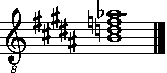
\includegraphics[height=1.15cm]{th-Bdim7.cropped} & Max. tense. All minor 3rds. \\
\rowcolor{rowB}
\textbf{Bm7$\flat$5} & B half-dim. & 1 -- $\flat$3 -- $\flat$5 -- $\flat$7 & 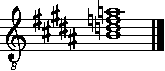
\includegraphics[height=1.15cm]{th-Bm7b5.cropped} & Tense, jazzy (also: B\o). \\
\bottomrule
\end{longtable}

\subsection*{The C Family}
\noindent\textbf{Key signature:} no sharps or flats.\smallskip

\begin{center}
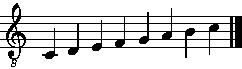
\includegraphics[height=1.15cm]{scale-C.cropped}\\[2pt]
{\small\color{mygray}\textbf{1} C\quad \textbf{2} D\quad \textbf{3} E\quad \textbf{4} F\quad \textbf{5} G\quad \textbf{6} A\quad \textbf{7} B\quad \textbf{8} C}
\end{center}

\begin{longtable}{@{}l l l c >{\raggedright\arraybackslash}p{4.4cm}@{}}
\toprule
\textbf{Symbol} & \textbf{Full name} & \textbf{Formula} & \textbf{Staff} & \textbf{Colour / use} \\
\midrule\endhead
\rowcolor{rowA}
\textbf{C} & C major & 1 -- 3 -- 5 & 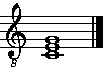
\includegraphics[height=1.15cm]{th-Cmaj.cropped} & Bright, stable. \\
\rowcolor{rowB}
\textbf{Cm} & C minor & 1 -- $\flat$3 -- 5 & 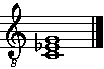
\includegraphics[height=1.15cm]{th-Cm.cropped} & Dark. Lower the 3rd: E $\to$ E$\flat$. \\
\rowcolor{rowA}
\textbf{C5} & C power chord & 1 -- 5 & 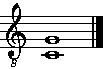
\includegraphics[height=1.15cm]{th-C5.cropped} & Raw, neutral. No 3rd. \\
\rowcolor{rowB}
\textbf{Csus2} & C sus. 2nd & 1 -- 2 -- 5 & 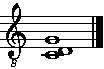
\includegraphics[height=1.15cm]{th-Csus2.cropped} & Open. Replace 3rd with 2nd (D). \\
\rowcolor{rowA}
\textbf{Csus4} & C sus. 4th & 1 -- 4 -- 5 & 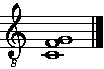
\includegraphics[height=1.15cm]{th-Csus4.cropped} & Tense. Replace 3rd with 4th (F). \\
\rowcolor{rowB}
\textbf{C6} & C major sixth & 1 -- 3 -- 5 -- 6 & 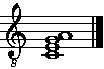
\includegraphics[height=1.15cm]{th-C6.cropped} & Sweet, vintage. Add 6th (A). \\
\rowcolor{rowA}
\textbf{Cadd9} & C add nine & 1 -- 3 -- 5 -- 9 & 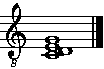
\includegraphics[height=1.15cm]{th-Cadd9.cropped} & Colourful. Add 2nd/9th (D), no 7th. \\
\rowcolor{rowB}
\textbf{C7} & C dominant 7th & 1 -- 3 -- 5 -- $\flat$7 & 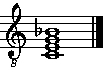
\includegraphics[height=1.15cm]{th-C7.cropped} & Bluesy. Lower 7th: B $\to$ B$\flat$. \\
\rowcolor{rowA}
\textbf{Cmaj7} & C major 7th & 1 -- 3 -- 5 -- 7 & 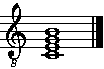
\includegraphics[height=1.15cm]{th-Cmaj7.cropped} & Dreamy, jazzy. Keep natural 7th (B). \\
\rowcolor{rowB}
\textbf{Cm7} & C minor 7th & 1 -- $\flat$3 -- 5 -- $\flat$7 & 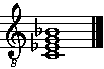
\includegraphics[height=1.15cm]{th-Cm7.cropped} & Mellow, soulful. Lower 3rd and 7th. \\
\rowcolor{rowA}
\textbf{Caug} & C augmented & 1 -- 3 -- $\sharp$5 & 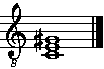
\includegraphics[height=1.15cm]{th-Caug.cropped} & Eerie. Raise the 5th by 1 semitone. \\
\rowcolor{rowB}
\textbf{Cdim} & C diminished & 1 -- $\flat$3 -- $\flat$5 & 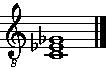
\includegraphics[height=1.15cm]{th-Cdim.cropped} & Very tense. Lower 3rd and 5th. \\
\rowcolor{rowA}
\textbf{Cdim7} & C dim. 7th & 1 -- $\flat$3 -- $\flat$5 -- $\flat\flat$7 & 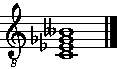
\includegraphics[height=1.15cm]{th-Cdim7.cropped} & Max. tense. All minor 3rds. \\
\rowcolor{rowB}
\textbf{Cm7$\flat$5} & C half-dim. & 1 -- $\flat$3 -- $\flat$5 -- $\flat$7 & 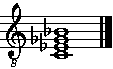
\includegraphics[height=1.15cm]{th-Cm7b5.cropped} & Tense, jazzy (also: C\o). \\
\bottomrule
\end{longtable}

\subsection*{The D Family}
\noindent\textbf{Key signature:} two sharps: F$\sharp$, C$\sharp$.\smallskip

\begin{center}
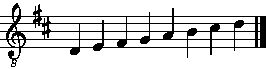
\includegraphics[height=1.15cm]{scale-D.cropped}\\[2pt]
{\small\color{mygray}\textbf{1} D\quad \textbf{2} E\quad \textbf{3} F$\sharp$\quad \textbf{4} G\quad \textbf{5} A\quad \textbf{6} B\quad \textbf{7} C$\sharp$\quad \textbf{8} D}
\end{center}

\begin{longtable}{@{}l l l c >{\raggedright\arraybackslash}p{4.4cm}@{}}
\toprule
\textbf{Symbol} & \textbf{Full name} & \textbf{Formula} & \textbf{Staff} & \textbf{Colour / use} \\
\midrule\endhead
\rowcolor{rowA}
\textbf{D} & D major & 1 -- 3 -- 5 & 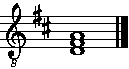
\includegraphics[height=1.15cm]{th-Dmaj.cropped} & Bright, stable. \\
\rowcolor{rowB}
\textbf{Dm} & D minor & 1 -- $\flat$3 -- 5 & 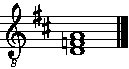
\includegraphics[height=1.15cm]{th-Dm.cropped} & Dark. Lower the 3rd: F$\sharp$ $\to$ F. \\
\rowcolor{rowA}
\textbf{D5} & D power chord & 1 -- 5 & 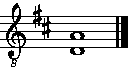
\includegraphics[height=1.15cm]{th-D5.cropped} & Raw, neutral. No 3rd. \\
\rowcolor{rowB}
\textbf{Dsus2} & D sus. 2nd & 1 -- 2 -- 5 & 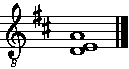
\includegraphics[height=1.15cm]{th-Dsus2.cropped} & Open. Replace 3rd with 2nd (E). \\
\rowcolor{rowA}
\textbf{Dsus4} & D sus. 4th & 1 -- 4 -- 5 & 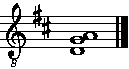
\includegraphics[height=1.15cm]{th-Dsus4.cropped} & Tense. Replace 3rd with 4th (G). \\
\rowcolor{rowB}
\textbf{D6} & D major sixth & 1 -- 3 -- 5 -- 6 & 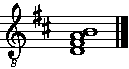
\includegraphics[height=1.15cm]{th-D6.cropped} & Sweet, vintage. Add 6th (B). \\
\rowcolor{rowA}
\textbf{Dadd9} & D add nine & 1 -- 3 -- 5 -- 9 & 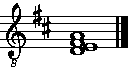
\includegraphics[height=1.15cm]{th-Dadd9.cropped} & Colourful. Add 2nd/9th (E), no 7th. \\
\rowcolor{rowB}
\textbf{D7} & D dominant 7th & 1 -- 3 -- 5 -- $\flat$7 & 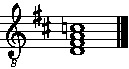
\includegraphics[height=1.15cm]{th-D7.cropped} & Bluesy. Lower 7th: C$\sharp$ $\to$ C. \\
\rowcolor{rowA}
\textbf{Dmaj7} & D major 7th & 1 -- 3 -- 5 -- 7 & 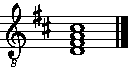
\includegraphics[height=1.15cm]{th-Dmaj7.cropped} & Dreamy, jazzy. Keep natural 7th (C$\sharp$). \\
\rowcolor{rowB}
\textbf{Dm7} & D minor 7th & 1 -- $\flat$3 -- 5 -- $\flat$7 & 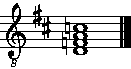
\includegraphics[height=1.15cm]{th-Dm7.cropped} & Mellow, soulful. Lower 3rd and 7th. \\
\rowcolor{rowA}
\textbf{Daug} & D augmented & 1 -- 3 -- $\sharp$5 & 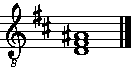
\includegraphics[height=1.15cm]{th-Daug.cropped} & Eerie. Raise the 5th by 1 semitone. \\
\rowcolor{rowB}
\textbf{Ddim} & D diminished & 1 -- $\flat$3 -- $\flat$5 & 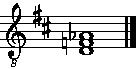
\includegraphics[height=1.15cm]{th-Ddim.cropped} & Very tense. Lower 3rd and 5th. \\
\rowcolor{rowA}
\textbf{Ddim7} & D dim. 7th & 1 -- $\flat$3 -- $\flat$5 -- $\flat\flat$7 & 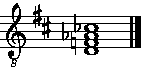
\includegraphics[height=1.15cm]{th-Ddim7.cropped} & Max. tense. All minor 3rds. \\
\rowcolor{rowB}
\textbf{Dm7$\flat$5} & D half-dim. & 1 -- $\flat$3 -- $\flat$5 -- $\flat$7 & 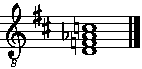
\includegraphics[height=1.15cm]{th-Dm7b5.cropped} & Tense, jazzy (also: D\o). \\
\bottomrule
\end{longtable}

\subsection*{The E Family}
\noindent\textbf{Key signature:} four sharps: F$\sharp$, C$\sharp$, G$\sharp$, D$\sharp$.\smallskip

\begin{center}
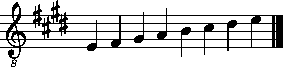
\includegraphics[height=1.15cm]{scale-E.cropped}\\[2pt]
{\small\color{mygray}\textbf{1} E\quad \textbf{2} F$\sharp$\quad \textbf{3} G$\sharp$\quad \textbf{4} A\quad \textbf{5} B\quad \textbf{6} C$\sharp$\quad \textbf{7} D$\sharp$\quad \textbf{8} E}
\end{center}

\begin{longtable}{@{}l l l c >{\raggedright\arraybackslash}p{4.4cm}@{}}
\toprule
\textbf{Symbol} & \textbf{Full name} & \textbf{Formula} & \textbf{Staff} & \textbf{Colour / use} \\
\midrule\endhead
\rowcolor{rowA}
\textbf{E} & E major & 1 -- 3 -- 5 & 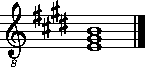
\includegraphics[height=1.15cm]{th-Emaj.cropped} & Bright, stable. \\
\rowcolor{rowB}
\textbf{Em} & E minor & 1 -- $\flat$3 -- 5 & 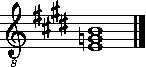
\includegraphics[height=1.15cm]{th-Em.cropped} & Dark. Lower the 3rd: G$\sharp$ $\to$ G. \\
\rowcolor{rowA}
\textbf{E5} & E power chord & 1 -- 5 & 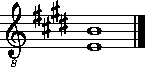
\includegraphics[height=1.15cm]{th-E5.cropped} & Raw, neutral. No 3rd. \\
\rowcolor{rowB}
\textbf{Esus2} & E sus. 2nd & 1 -- 2 -- 5 & 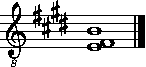
\includegraphics[height=1.15cm]{th-Esus2.cropped} & Open. Replace 3rd with 2nd (F$\sharp$). \\
\rowcolor{rowA}
\textbf{Esus4} & E sus. 4th & 1 -- 4 -- 5 & 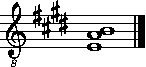
\includegraphics[height=1.15cm]{th-Esus4.cropped} & Tense. Replace 3rd with 4th (A). \\
\rowcolor{rowB}
\textbf{E6} & E major sixth & 1 -- 3 -- 5 -- 6 & 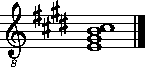
\includegraphics[height=1.15cm]{th-E6.cropped} & Sweet, vintage. Add 6th (C$\sharp$). \\
\rowcolor{rowA}
\textbf{Eadd9} & E add nine & 1 -- 3 -- 5 -- 9 & 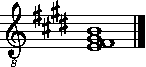
\includegraphics[height=1.15cm]{th-Eadd9.cropped} & Colourful. Add 2nd/9th (F$\sharp$), no 7th. \\
\rowcolor{rowB}
\textbf{E7} & E dominant 7th & 1 -- 3 -- 5 -- $\flat$7 & 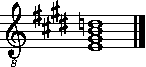
\includegraphics[height=1.15cm]{th-E7.cropped} & Bluesy. Lower 7th: D$\sharp$ $\to$ D. \\
\rowcolor{rowA}
\textbf{Emaj7} & E major 7th & 1 -- 3 -- 5 -- 7 & 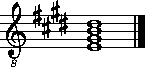
\includegraphics[height=1.15cm]{th-Emaj7.cropped} & Dreamy, jazzy. Keep natural 7th (D$\sharp$). \\
\rowcolor{rowB}
\textbf{Em7} & E minor 7th & 1 -- $\flat$3 -- 5 -- $\flat$7 & 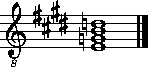
\includegraphics[height=1.15cm]{th-Em7.cropped} & Mellow, soulful. Lower 3rd and 7th. \\
\rowcolor{rowA}
\textbf{Eaug} & E augmented & 1 -- 3 -- $\sharp$5 & 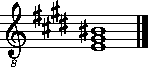
\includegraphics[height=1.15cm]{th-Eaug.cropped} & Eerie. Raise the 5th by 1 semitone. \\
\rowcolor{rowB}
\textbf{Edim} & E diminished & 1 -- $\flat$3 -- $\flat$5 & 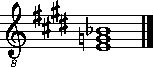
\includegraphics[height=1.15cm]{th-Edim.cropped} & Very tense. Lower 3rd and 5th. \\
\rowcolor{rowA}
\textbf{Edim7} & E dim. 7th & 1 -- $\flat$3 -- $\flat$5 -- $\flat\flat$7 & 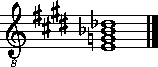
\includegraphics[height=1.15cm]{th-Edim7.cropped} & Max. tense. All minor 3rds. \\
\rowcolor{rowB}
\textbf{Em7$\flat$5} & E half-dim. & 1 -- $\flat$3 -- $\flat$5 -- $\flat$7 & 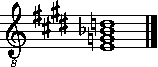
\includegraphics[height=1.15cm]{th-Em7b5.cropped} & Tense, jazzy (also: E\o). \\
\bottomrule
\end{longtable}

\subsection*{The F Family}
\noindent\textbf{Key signature:} one flat: B$\flat$.\smallskip

\begin{center}
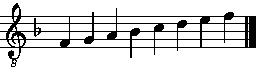
\includegraphics[height=1.15cm]{scale-F.cropped}\\[2pt]
{\small\color{mygray}\textbf{1} F\quad \textbf{2} G\quad \textbf{3} A\quad \textbf{4} B$\flat$\quad \textbf{5} C\quad \textbf{6} D\quad \textbf{7} E\quad \textbf{8} F}
\end{center}

\begin{longtable}{@{}l l l c >{\raggedright\arraybackslash}p{4.4cm}@{}}
\toprule
\textbf{Symbol} & \textbf{Full name} & \textbf{Formula} & \textbf{Staff} & \textbf{Colour / use} \\
\midrule\endhead
\rowcolor{rowA}
\textbf{F} & F major & 1 -- 3 -- 5 & 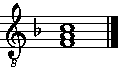
\includegraphics[height=1.15cm]{th-Fmaj.cropped} & Bright, stable. \\
\rowcolor{rowB}
\textbf{Fm} & F minor & 1 -- $\flat$3 -- 5 & 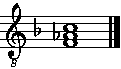
\includegraphics[height=1.15cm]{th-Fm.cropped} & Dark. Lower the 3rd: A $\to$ A$\flat$. \\
\rowcolor{rowA}
\textbf{F5} & F power chord & 1 -- 5 & 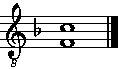
\includegraphics[height=1.15cm]{th-F5.cropped} & Raw, neutral. No 3rd. \\
\rowcolor{rowB}
\textbf{Fsus2} & F sus. 2nd & 1 -- 2 -- 5 & 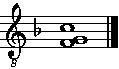
\includegraphics[height=1.15cm]{th-Fsus2.cropped} & Open. Replace 3rd with 2nd (G). \\
\rowcolor{rowA}
\textbf{Fsus4} & F sus. 4th & 1 -- 4 -- 5 & 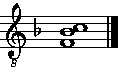
\includegraphics[height=1.15cm]{th-Fsus4.cropped} & Tense. Replace 3rd with 4th (B$\flat$). \\
\rowcolor{rowB}
\textbf{F6} & F major sixth & 1 -- 3 -- 5 -- 6 & 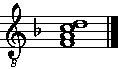
\includegraphics[height=1.15cm]{th-F6.cropped} & Sweet, vintage. Add 6th (D). \\
\rowcolor{rowA}
\textbf{Fadd9} & F add nine & 1 -- 3 -- 5 -- 9 & 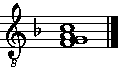
\includegraphics[height=1.15cm]{th-Fadd9.cropped} & Colourful. Add 2nd/9th (G), no 7th. \\
\rowcolor{rowB}
\textbf{F7} & F dominant 7th & 1 -- 3 -- 5 -- $\flat$7 & 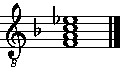
\includegraphics[height=1.15cm]{th-F7.cropped} & Bluesy. Lower 7th: E $\to$ E$\flat$. \\
\rowcolor{rowA}
\textbf{Fmaj7} & F major 7th & 1 -- 3 -- 5 -- 7 & 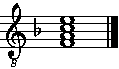
\includegraphics[height=1.15cm]{th-Fmaj7.cropped} & Dreamy, jazzy. Keep natural 7th (E). \\
\rowcolor{rowB}
\textbf{Fm7} & F minor 7th & 1 -- $\flat$3 -- 5 -- $\flat$7 & 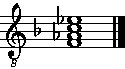
\includegraphics[height=1.15cm]{th-Fm7.cropped} & Mellow, soulful. Lower 3rd and 7th. \\
\rowcolor{rowA}
\textbf{Faug} & F augmented & 1 -- 3 -- $\sharp$5 & 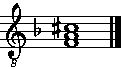
\includegraphics[height=1.15cm]{th-Faug.cropped} & Eerie. Raise the 5th by 1 semitone. \\
\rowcolor{rowB}
\textbf{Fdim} & F diminished & 1 -- $\flat$3 -- $\flat$5 & 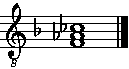
\includegraphics[height=1.15cm]{th-Fdim.cropped} & Very tense. Lower 3rd and 5th. \\
\rowcolor{rowA}
\textbf{Fdim7} & F dim. 7th & 1 -- $\flat$3 -- $\flat$5 -- $\flat\flat$7 & 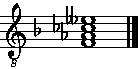
\includegraphics[height=1.15cm]{th-Fdim7.cropped} & Max. tense. All minor 3rds. \\
\rowcolor{rowB}
\textbf{Fm7$\flat$5} & F half-dim. & 1 -- $\flat$3 -- $\flat$5 -- $\flat$7 & 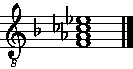
\includegraphics[height=1.15cm]{th-Fm7b5.cropped} & Tense, jazzy (also: F\o). \\
\bottomrule
\end{longtable}

\subsection*{The G Family}
\noindent\textbf{Key signature:} one sharp: F$\sharp$.\smallskip

\begin{center}
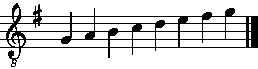
\includegraphics[height=1.15cm]{scale-G.cropped}\\[2pt]
{\small\color{mygray}\textbf{1} G\quad \textbf{2} A\quad \textbf{3} B\quad \textbf{4} C\quad \textbf{5} D\quad \textbf{6} E\quad \textbf{7} F$\sharp$\quad \textbf{8} G}
\end{center}

\begin{longtable}{@{}l l l c >{\raggedright\arraybackslash}p{4.4cm}@{}}
\toprule
\textbf{Symbol} & \textbf{Full name} & \textbf{Formula} & \textbf{Staff} & \textbf{Colour / use} \\
\midrule\endhead
\rowcolor{rowA}
\textbf{G} & G major & 1 -- 3 -- 5 & 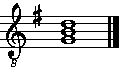
\includegraphics[height=1.15cm]{th-Gmaj.cropped} & Bright, stable. \\
\rowcolor{rowB}
\textbf{Gm} & G minor & 1 -- $\flat$3 -- 5 & 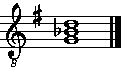
\includegraphics[height=1.15cm]{th-Gm.cropped} & Dark. Lower the 3rd: B $\to$ B$\flat$. \\
\rowcolor{rowA}
\textbf{G5} & G power chord & 1 -- 5 & 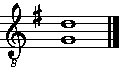
\includegraphics[height=1.15cm]{th-G5.cropped} & Raw, neutral. No 3rd. \\
\rowcolor{rowB}
\textbf{Gsus2} & G sus. 2nd & 1 -- 2 -- 5 & 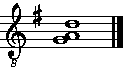
\includegraphics[height=1.15cm]{th-Gsus2.cropped} & Open. Replace 3rd with 2nd (A). \\
\rowcolor{rowA}
\textbf{Gsus4} & G sus. 4th & 1 -- 4 -- 5 & 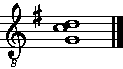
\includegraphics[height=1.15cm]{th-Gsus4.cropped} & Tense. Replace 3rd with 4th (C). \\
\rowcolor{rowB}
\textbf{G6} & G major sixth & 1 -- 3 -- 5 -- 6 & 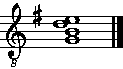
\includegraphics[height=1.15cm]{th-G6.cropped} & Sweet, vintage. Add 6th (E). \\
\rowcolor{rowA}
\textbf{Gadd9} & G add nine & 1 -- 3 -- 5 -- 9 & 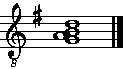
\includegraphics[height=1.15cm]{th-Gadd9.cropped} & Colourful. Add 2nd/9th (A), no 7th. \\
\rowcolor{rowB}
\textbf{G7} & G dominant 7th & 1 -- 3 -- 5 -- $\flat$7 & 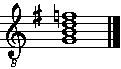
\includegraphics[height=1.15cm]{th-G7.cropped} & Bluesy. Lower 7th: F$\sharp$ $\to$ F. \\
\rowcolor{rowA}
\textbf{Gmaj7} & G major 7th & 1 -- 3 -- 5 -- 7 & 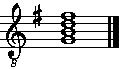
\includegraphics[height=1.15cm]{th-Gmaj7.cropped} & Dreamy, jazzy. Keep natural 7th (F$\sharp$). \\
\rowcolor{rowB}
\textbf{Gm7} & G minor 7th & 1 -- $\flat$3 -- 5 -- $\flat$7 & 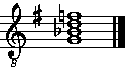
\includegraphics[height=1.15cm]{th-Gm7.cropped} & Mellow, soulful. Lower 3rd and 7th. \\
\rowcolor{rowA}
\textbf{Gaug} & G augmented & 1 -- 3 -- $\sharp$5 & 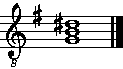
\includegraphics[height=1.15cm]{th-Gaug.cropped} & Eerie. Raise the 5th by 1 semitone. \\
\rowcolor{rowB}
\textbf{Gdim} & G diminished & 1 -- $\flat$3 -- $\flat$5 & 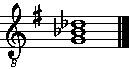
\includegraphics[height=1.15cm]{th-Gdim.cropped} & Very tense. Lower 3rd and 5th. \\
\rowcolor{rowA}
\textbf{Gdim7} & G dim. 7th & 1 -- $\flat$3 -- $\flat$5 -- $\flat\flat$7 & 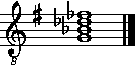
\includegraphics[height=1.15cm]{th-Gdim7.cropped} & Max. tense. All minor 3rds. \\
\rowcolor{rowB}
\textbf{Gm7$\flat$5} & G half-dim. & 1 -- $\flat$3 -- $\flat$5 -- $\flat$7 & 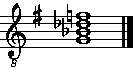
\includegraphics[height=1.15cm]{th-Gm7b5.cropped} & Tense, jazzy (also: G\o). \\
\bottomrule
\end{longtable}


\label{fin-theorie}

% ====================================================================
\newpage
\section{Open-Position Major Chords}
\label{deb-diagrammes}

\begin{chordrow}
\cw{E}{\chord{E}{1}{1/o,5/o,6/o}{}{2/2,3/2,4/1}} &
\cw{A}{\chord{A}{1}{1/x,2/o,6/o}{}{3/2,4/2,5/2}} &
\cw{D}{\chord{D}{1}{1/x,2/x,3/o}{}{4/2,5/3,6/2}} &
\cw{G}{\chord{G}{1}{3/o,4/o,5/o}{}{1/3,2/2,6/3}} &
\cw{C}{\chord{C}{1}{1/x,4/o,6/o}{}{2/3,3/2,5/1}} &
\cw{F}{\chord{F}{1}{}{1/6/1}{2/3,3/3,4/2}}
\end{chordrow}
\noindent{\small\color{mygray}%
\textbf{E} 022100\quad \textbf{A} x02220\quad \textbf{D} xx0232\quad
\textbf{G} 320003\quad \textbf{C} x32010\quad \textbf{F} 133211 (barre at fret~1)}

% ====================================================================
\section{Open-Position Minor Chords}

\begin{chordrow}
\cw{Em}{\chord{Em}{1}{1/o,4/o,5/o,6/o}{}{2/2,3/2}} &
\cw{Am}{\chord{Am}{1}{1/x,2/o,6/o}{}{3/2,4/2,5/1}} &
\cw{Dm}{\chord{Dm}{1}{1/x,2/x,3/o}{}{4/2,5/3,6/1}} &
\cw{Fm}{\chord{Fm}{1}{}{1/6/1}{2/3,3/3}} &
\cw{Bm}{\chord{Bm}{2}{1/x}{2/6/1}{3/3,4/3,5/2}} & \\
\end{chordrow}
\noindent{\small\color{mygray}%
\textbf{Em} 022000\quad \textbf{Am} x02210\quad \textbf{Dm} xx0231\quad
\textbf{Fm} 133111 (barre at 1)\quad \textbf{Bm} x24432 (barre at 2)}

% ====================================================================
\section{Dominant 7th Chords}
\noindent{\small 1 -- 3 -- 5 -- $\flat$7: bluesy and tense, naturally resolving to the tonic.}\smallskip

\begin{chordrow}
\cw{E7}{\chord{E7}{1}{1/o,3/o,5/o,6/o}{}{2/2,4/1}} &
\cw{A7}{\chord{A7}{1}{1/x,2/o,4/o,6/o}{}{3/2,5/2}} &
\cw{D7}{\chord{D7}{1}{1/x,2/x,3/o}{}{4/2,5/1,6/2}} &
\cw{G7}{\chord{G7}{1}{3/o,4/o,5/o}{}{1/3,2/2,6/1}} &
\cw{C7}{\chord{C7}{1}{1/x,6/o}{}{2/3,3/2,4/3,5/1}} &
\cw{B7}{\chord{B7}{1}{1/x,5/o}{}{2/2,3/1,4/2,6/2}}
\end{chordrow}
\noindent{\small\color{mygray}%
\textbf{E7} 020100\quad \textbf{A7} x02020\quad \textbf{D7} xx0212\quad
\textbf{G7} 320001\quad \textbf{C7} x32310\quad \textbf{B7} x21202}

% ====================================================================
\section{Major 7th Chords (maj7)}
\noindent{\small 1 -- 3 -- 5 -- 7: smooth, dreamy and jazzy.}\smallskip

\begin{chordrow}
\cw{Cmaj7}{\chord{Cmaj7}{1}{1/x,4/o,5/o,6/o}{}{2/3,3/2}} &
\cw{Dmaj7}{\chord{Dmaj7}{1}{1/x,2/x,3/o}{}{4/2,5/2,6/2}} &
\cw{Emaj7}{\chord{Emaj7}{1}{1/o,5/o,6/o}{}{2/2,3/1,4/1}} &
\cw{Amaj7}{\chord{Amaj7}{1}{1/x,2/o,6/o}{}{3/2,4/1,5/2}} &
\cw{Gmaj7}{\chord{Gmaj7}{1}{3/o,4/o,5/o}{}{1/3,2/2,6/2}} &
\cw{Fmaj7}{\chord{Fmaj7}{1}{1/x,2/x,6/o}{}{3/3,4/2,5/1}}
\end{chordrow}
\noindent{\small\color{mygray}%
\textbf{Cmaj7} x32000\quad \textbf{Dmaj7} xx0222\quad \textbf{Emaj7} 021100\quad
\textbf{Amaj7} x02120\quad \textbf{Gmaj7} 320002\quad \textbf{Fmaj7} xx3210}

% ====================================================================
\section{Minor 7th Chords (m7)}
\noindent{\small 1 -- $\flat$3 -- 5 -- $\flat$7: cornerstone of jazz, soul and R\&B.}\smallskip

\begin{chordrow}
\cw{Em7}{\chord{Em7}{1}{1/o,3/o,4/o,5/o,6/o}{}{2/2}} &
\cw{Am7}{\chord{Am7}{1}{1/x,2/o,4/o,6/o}{}{3/2,5/1}} &
\cw{Dm7}{\chord{Dm7}{1}{1/x,2/x,3/o}{}{4/2,5/1,6/1}} &
\cw{Bm7}{\chord{Bm7}{2}{1/x}{2/6/1}{3/3,5/2}} & & \\
\end{chordrow}
\noindent{\small\color{mygray}%
\textbf{Em7} 020000\quad \textbf{Am7} x02010\quad \textbf{Dm7} xx0211\quad
\textbf{Bm7} x24232 (barre at 2, variant shown)}

% ====================================================================
\section{Suspended Chords (sus2, sus4)}
\noindent{\small The 3rd is replaced by a 2nd or 4th: harmony is open and unresolved.}\smallskip

\begin{chordrow}
\cw{Dsus2}{\chord{Dsus2}{1}{1/x,2/x,3/o,6/o}{}{4/2,5/3}} &
\cw{Dsus4}{\chord{Dsus4}{1}{1/x,2/x,3/o}{}{4/2,5/3,6/3}} &
\cw{Asus2}{\chord{Asus2}{1}{1/x,2/o,5/o,6/o}{}{3/2,4/2}} &
\cw{Asus4}{\chord{Asus4}{1}{1/x,2/o,6/o}{}{3/2,4/2,5/3}} &
\cw{Esus4}{\chord{Esus4}{1}{1/o,5/o,6/o}{}{2/2,3/2,4/2}} & \\
\end{chordrow}
\noindent{\small\color{mygray}%
\textbf{Dsus2} xx0230\quad \textbf{Dsus4} xx0233\quad \textbf{Asus2} x02200\quad
\textbf{Asus4} x02230\quad \textbf{Esus4} 022200}

% ====================================================================
\section{Power Chords (5th Chords)}
\noindent{\small 1 -- 5 only, no 3rd: neither major nor minor. Essential in rock and metal.}\smallskip

\begin{chordrow}
\cw{E5}{\chord{E5}{1}{1/o,4/x,5/x,6/x}{}{2/2,3/2}} &
\cw{A5}{\chord{A5}{1}{1/x,2/o,5/x,6/x}{}{3/2,4/2}} &
\cw{D5}{\chord{D5}{1}{1/x,2/x,3/o,6/x}{}{4/2,5/3}} &
\cw{G5}{\chord{G5}{3}{4/x,5/x,6/x}{}{1/1,2/3,3/3}} & & \\
\end{chordrow}
\noindent{\small\color{mygray}%
\textbf{E5} 022xxx\quad \textbf{A5} x022xx\quad \textbf{D5} xx023x\quad
\textbf{G5} 355xxx (movable E5-shape at fret~3)}

% ====================================================================
\section{Barre Chords --- E Shape (Major and Minor)}
\noindent{\small Open E or Em shape moved up the neck.
Index finger barres all 6 strings; fret number at left = root.}\smallskip

\begin{chordrow}
\cw{F_E}{\chord{F}{1}{}{1/6/1}{2/3,3/3,4/2}} &
\cw{G_E}{\chord{G}{3}{}{1/6/1}{2/3,3/3,4/2}} &
\cw{A_E}{\chord{A}{5}{}{1/6/1}{2/3,3/3,4/2}} &
\cw{B_E}{\chord{B}{7}{}{1/6/1}{2/3,3/3,4/2}} &
\cw{Fm_E}{\chord{Fm}{1}{}{1/6/1}{2/3,3/3}} &
\cw{Bm_E}{\chord{Bm}{2}{1/x}{2/6/1}{3/3,4/3,5/2}}
\end{chordrow}
\noindent{\small\color{mygray}%
Major: fret 1=F, 2=F\#, 3=G, 5=A, 7=B, 8=C, 10=D\ldots\quad
Minor: fret 1=Fm, 2=F\#m, 5=Am, 7=Bm\ldots}

% ====================================================================
\section{Barre Chords --- A Shape (Major and Minor)}
\noindent{\small Open A or Am shape moved up the neck.
Index finger barres strings~2--6.}\smallskip

\begin{chordrow}
\cw{Bb_A}{\chord{B$\flat$}{1}{1/x}{2/6/1}{3/3,4/3,5/3}} &
\cw{B_A}{\chord{B}{2}{1/x}{2/6/1}{3/3,4/3,5/3}} &
\cw{C_A}{\chord{C}{3}{1/x}{2/6/1}{3/3,4/3,5/3}} &
\cw{Bbm_A}{\chord{B$\flat$m}{1}{1/x}{2/6/1}{3/3,4/3,5/2}} &
\cw{Bm_A}{\chord{Bm}{2}{1/x}{2/6/1}{3/3,4/3,5/2}} &
\cw{Cm_A}{\chord{Cm}{3}{1/x}{2/6/1}{3/3,4/3,5/2}}
\end{chordrow}
\noindent{\small\color{mygray}%
Major: fret 1=B$\flat$, 2=B, 3=C, 5=D, 7=E, 10=G\ldots\quad
Minor: fret 1=B$\flat$m, 2=Bm, 3=Cm, 5=Dm\ldots}

% ====================================================================
\section{Added-Tone Chords (add9, add6)}
\noindent{\small Triad + extra colour note (9th or 6th), without a 7th.}\smallskip

\begin{chordrow}
\cw{Cadd9}{\chord{Cadd9}{1}{1/x,4/o}{}{2/3,3/2,5/3,6/3}} &
\cw{Dadd9}{\chord{Dadd9}{2}{1/x,6/o}{}{2/4,3/3,4/1,5/2}} &
\cw{Eadd9}{\chord{Eadd9}{1}{1/o,5/o,6/o}{}{2/2,3/4,4/1}} &
\cw{D6}{\chord{D6}{1}{1/x,2/x,3/o,5/o}{}{4/2,6/2}} &
\cw{A6}{\chord{A6}{1}{1/x,2/o}{}{3/2,4/2,5/2,6/2}} & \\
\end{chordrow}
\noindent{\small\color{mygray}%
\textbf{Cadd9} x32033\quad \textbf{Dadd9} x54230\quad \textbf{Eadd9} 024100\quad
\textbf{D6} xx0202\quad \textbf{A6} x02222}

% ====================================================================
\section{Augmented Chords (aug)}
\noindent{\small 1 -- 3 -- \#5: eerie and tense. Symmetrical --- repeats every 4 semitones.}\smallskip

\begin{chordrow}
\cw{Eaug}{\chord{Eaug}{1}{1/o,6/o}{}{2/3,3/2,4/1,5/1}} &
\cw{Aaug}{\chord{Aaug}{1}{1/x,2/o}{}{3/3,4/2,5/2,6/1}} &
\cw{Caug}{\chord{Caug}{1}{1/x,6/o}{}{2/3,3/2,4/1,5/1}} & & & \\
\end{chordrow}
\noindent{\small\color{mygray}%
\textbf{Eaug} 032110\quad \textbf{Aaug} x03221\quad \textbf{Caug} x32110\quad
Eaug = G\#aug = Caug (same pitch-class set).}

% ====================================================================
\section{Diminished Chords (dim, dim7)}
\noindent{\small Stacked minor 3rds. A dim7 repeats every 3 semitones.}\smallskip

\begin{chordrow}
\cw{Bdim}{\chord{Bdim}{1}{1/x,6/x}{}{2/2,3/3,4/4,5/3}} &
\cw{Edim7}{\chord{Edim7}{1}{1/o,4/o,6/x}{}{2/1,3/2,5/2}} &
\cw{Adim7}{\chord{Adim7}{1}{1/x,2/o}{}{3/1,4/2,5/1,6/2}} & & & \\
\end{chordrow}
\noindent{\small\color{mygray}%
\textbf{Bdim} x2343x\quad \textbf{Edim7} 01202x\quad \textbf{Adim7} x01212\quad
Shift a dim7 up 3 frets to get the same chord on a new root.}

% ====================================================================
\section{Diatonic Chords and Roman Numeral Notation}

\noindent
Tonal music uses three complementary notation systems for chords.
Being able to move between them is an essential skill:

\medskip
\begin{center}\small\setlength{\tabcolsep}{0.7em}
\renewcommand{\arraystretch}{1.4}
\begin{tabular}{lp{9cm}}
\toprule
\textbf{System} & \textbf{Description} \\
\midrule
\textbf{Chord name} \newline (e.g.\ \textit{G, Am, Dm})
  & Gives the absolute pitch of the root and the chord quality
    (see the chord theory sections A--G).
    Useful for reading a chart or score. \\
\addlinespace
\textbf{Scale degrees} \newline (e.g.\ \textit{1, $\flat$3, 5})
  & Describes the \emph{internal structure} of a chord regardless of key.
    Used in the formula tables of this guide. \\
\addlinespace
\textbf{Roman numerals} \newline (e.g.\ \textit{I, IV, V, vi})
  & Indicates the \emph{position} of a chord within a given key:
    the numeral identifies the scale degree on which the chord is built.
    Upper case = major chord; lower case = minor chord;
    $^\circ$ = diminished chord.
    Useful for transposing a progression to any key. \\
\bottomrule
\end{tabular}
\end{center}

\subsection{The seven diatonic chords of a major key}

\noindent{\small
By stacking thirds on each degree of a major scale, we get seven chords
whose qualities always follow the same pattern:
\textbf{Maj -- min -- min -- Maj -- Maj -- min -- dim.}
The table below shows all three notations for the key of \textbf{C major}:}

\smallskip
\begin{chordrow}
\cw{C}{\chord{C}{1}{1/x,4/o,6/o}{}{2/3,3/2,5/1}} &
\cw{Dm}{\chord{Dm}{1}{1/x,2/x,3/o}{}{4/2,5/3,6/1}} &
\cw{Em}{\chord{Em}{1}{1/o,4/o,5/o,6/o}{}{2/2,3/2}} &
\cw{F}{\chord{F}{1}{}{1/6/1}{2/3,3/3,4/2}} &
\cw{G}{\chord{G}{1}{3/o,4/o,5/o}{}{1/3,2/2,6/3}} &
\cw{Am}{\chord{Am}{1}{1/x,2/o,6/o}{}{3/2,4/2,5/1}}
\end{chordrow}

\begin{center}\small\setlength{\tabcolsep}{0.6em}
\renewcommand{\arraystretch}{1.4}
\begin{tabular}{lccccccc}
\toprule
  & \textbf{I} & \textbf{ii} & \textbf{iii}
  & \textbf{IV} & \textbf{V} & \textbf{vi} & \textbf{vii}$^\circ$ \\
\midrule
\textit{C major} & C  & Dm  & Em   & F  & G  & Am  & Bdim  \\
\textit{G major} & G  & Am  & Bm   & C  & D  & Em  & F\#dim \\
\textit{D major} & D  & Em  & F\#m & G  & A  & Bm  & C\#dim \\
\textit{A major} & A  & Bm  & C\#m & D  & E  & F\#m & G\#dim \\
\textit{E major} & E  & F\#m & G\#m & A  & B  & C\#m & D\#dim \\
\bottomrule
\end{tabular}
\end{center}

\smallskip
\noindent{\small\color{mygray}
\textit{How to use this table:} identify the Roman numeral pattern of a
progression, then read across the row for the desired key.
Example: \textbf{I -- V -- vi -- IV} in C = C -- G -- Am -- F;
in G = G -- D -- Em -- C; in D = D -- A -- Bm -- G.}

\subsection{Common progressions and their Roman numeral patterns}

\noindent{\small
The progressions below appear in thousands of songs.
The column \textit{In C} gives the literal chord names;
\textit{Song} shows the actual key used in the recording.}

\medskip
\begin{center}\small\setlength{\tabcolsep}{0.55em}
\renewcommand{\arraystretch}{1.3}
\begin{tabular}{llll}
\toprule
\textbf{Roman pattern} & \textbf{In C}
  & \textbf{Song (key)} & \textbf{Feel} \\
\midrule
I -- IV -- V
  & C -- F -- G        & La Bamba (A)                   & Bright, driving \\
I -- V -- vi -- IV
  & C -- G -- Am -- F  & Let It Be (C)                  & Epic, universal \\
vi -- IV -- I -- V
  & Am -- F -- C -- G  & Zombie (Em)                    & Melancholic, rock \\
i -- VII -- VI -- VII
  & Am -- G -- F -- G  & All Along the Watchtower (C\#m) & Dramatic \\
I -- V -- vi -- iii -- IV
  & C -- G -- Am -- Em -- F & Pachelbel's Canon          & Timeless, classical \\
ii -- V -- I
  & Dm -- G -- C       & Jazz standard (C)              & Tension$\to$release \\
\bottomrule
\end{tabular}
\end{center}

% ====================================================================
\section{Chord Formula Quick Reference}

\begin{center}\small\setlength{\tabcolsep}{0.7em}
\renewcommand{\arraystretch}{1.35}
\begin{tabular}{llll}
\toprule
\textbf{Symbol suffix} & \textbf{Formula} &
\textbf{Semitone gaps} & \textbf{Character}\\
\midrule
(none) = Major      & 1 -- 3 -- 5              & +4, +3          & Bright, stable\\
m = Minor           & 1 -- $\flat$3 -- 5        & +3, +4          & Dark, melancholic\\
7 = Dom.\ 7th       & 1 -- 3 -- 5 -- $\flat$7   & +4, +3, +3      & Tense, bluesy\\
maj7                & 1 -- 3 -- 5 -- 7          & +4, +3, +4      & Dreamy, jazzy\\
m7                  & 1 -- $\flat$3 -- 5 -- $\flat$7 & +3, +4, +3 & Mellow, soulful\\
sus2                & 1 -- 2 -- 5              & +2, +5          & Open, floating\\
sus4                & 1 -- 4 -- 5              & +5, +2          & Tense, anticipating\\
5 = Power           & 1 -- 5                   & +7              & Raw, neutral\\
aug                 & 1 -- 3 -- $\sharp$5       & +4, +4          & Eerie, tense\\
dim                 & 1 -- $\flat$3 -- $\flat$5 & +3, +3          & Very tense\\
dim7                & 1 -- $\flat$3 -- $\flat$5 -- $\flat\flat$7 & +3,+3,+3 & Maximally tense\\
add9                & 1 -- 3 -- 5 -- 9         & triad + 9th     & Colourful, modern\\
6                   & 1 -- 3 -- 5 -- 6         & triad + 6th     & Sweet, vintage\\
\bottomrule
\end{tabular}
\end{center}

% ====================================================================
\label{fin-diagrammes}
\section{Strumming and Rhythm Basics}
\label{deb-pratique}

\noindent
\textbf{Strumming} is the act of sweeping the pick (or fingernails)
across several strings at once to produce a chord.
Two ingredients define a strumming pattern: the \textbf{time signature}
(how beats are grouped) and the \textbf{stroke direction}
(down or up) on each subdivision.

\subsection{Time signatures}

\begin{center}\small\setlength{\tabcolsep}{0.7em}\renewcommand{\arraystretch}{1.4}
\begin{tabular}{cll}
\toprule
\textbf{Sig.} & \textbf{Meaning} & \textbf{Feel / typical use} \\
\midrule
4/4 & 4 beats per bar, quarter note = 1 beat
    & Most pop, rock, blues --- the default \\
3/4 & 3 beats per bar
    & Waltz, ballads (e.g.\ ``Iris'' by Goo Goo Dolls) \\
6/8 & 6 eighth-note beats per bar, grouped 3+3
    & Compound feel; suits fingerpicking (e.g.\ ``House of the Rising Sun'') \\
\bottomrule
\end{tabular}
\end{center}

\subsection{Stroke notation}

\noindent
Strumming patterns in this guide use the following symbols:

\medskip
\begin{center}\small\setlength{\tabcolsep}{1.0em}\renewcommand{\arraystretch}{1.4}
\begin{tabular}{c>{\raggedright\arraybackslash}p{0.8\linewidth}}
\toprule
\textbf{Symbol} & \textbf{Meaning} \\
\midrule
\textbf{D} & Downstroke --- sweep from string 6 (low E) toward string 1 (high e) \\
\textbf{U} & Upstroke --- sweep from string 1 toward string 6 \\
\textbf{-} & Rest / lift --- do not strike the strings on this subdivision \\
\textbf{$\times$} & Choked strum --- touch the strings with the palm or fretting hand
                    to mute them just before or just as you strum \\
\bottomrule
\end{tabular}
\end{center}

\subsection{Counting subdivisions in 4/4}

\noindent
In 4/4 time, each beat can be divided into two eighth notes,
counted \textbf{1 and 2 and 3 and 4 and}.
Downstrokes fall on the numbered beats; upstrokes on the ``ands'':

\medskip
\begin{center}\small
\setlength{\tabcolsep}{0.0em}
\renewcommand{\arraystretch}{1.3}
\newcommand{\B}[1]{\textbf{#1}}  % bold beat
\begin{tabular}{*{8}{p{1.5cm}}}
\multicolumn{1}{c}{\B{1}} & \multicolumn{1}{c}{+}
& \multicolumn{1}{c}{\B{2}} & \multicolumn{1}{c}{+}
& \multicolumn{1}{c}{\B{3}} & \multicolumn{1}{c}{+}
& \multicolumn{1}{c}{\B{4}} & \multicolumn{1}{c}{+} \\
\hline
\multicolumn{1}{|c|}{\B{D}} & \multicolumn{1}{c|}{U}
& \multicolumn{1}{c|}{\B{D}} & \multicolumn{1}{c|}{U}
& \multicolumn{1}{c|}{\B{D}} & \multicolumn{1}{c|}{U}
& \multicolumn{1}{c|}{\B{D}} & \multicolumn{1}{c|}{U} \\
\hline
\end{tabular}\\[4pt]
{\color{mygray}\small All-eighth pattern: the simplest full 4/4 strum.}
\end{center}

\subsection{Common patterns}

\noindent
The table below shows the most widely used patterns.
Each cell is one eighth-note subdivision (``1 + 2 + 3 + 4 +'').
\textbf{Bold} = on-beat stroke; regular = off-beat (``and'') stroke.

\medskip
\begin{center}\small
\setlength{\tabcolsep}{0.55em}
\renewcommand{\arraystretch}{1.45}
\begin{tabular}{lccccccccl}
\toprule
\textbf{Pattern name} &
  \multicolumn{8}{c}{\textbf{Subdivisions: 1 + 2 + 3 + 4 +}} &
  \textbf{Used in} \\
\midrule
All down (4/4)
  & \textbf{D} & & \textbf{D} & & \textbf{D} & & \textbf{D} &
  & Folk, slow ballads \\
Basic 8ths
  & \textbf{D} & U & \textbf{D} & U & \textbf{D} & U & \textbf{D} & U
  & Pop, rock \\
Island / Reggae
  & \textbf{D} & \textbf{D} & U & \textbf{D} & U & \textbf{D} & U &
  & Bob Dylan, America \\
Pop ``4-chord''
  & \textbf{D} & U & \textbf{D} & U & - & U & \textbf{D} & U
  & Knockin', most pop \\
Oasis pattern
  & \textbf{D} & \textbf{D} & U & - & U & \textbf{D} & U &
  & Wonderwall, britpop \\
\bottomrule
\end{tabular}
\end{center}

\smallskip
\noindent{\small\color{mygray}
\textit{Reading tip:} always tap your foot on beats 1, 2, 3, 4.
Downstrokes align with foot taps; upstrokes happen as the foot rises.
Start very slowly with a metronome and only increase tempo once
the pattern is automatic.}

\subsection{Dynamics and accents}

\noindent{\small
A flat sequence of D and U strokes sounds mechanical.
Two techniques add life:

\begin{itemize}[nosep, leftmargin=1.4em]
  \item \textbf{Accent beats 2 and 4.} In most Western popular music,
    the snare drum lands on beats 2 and 4 (the ``backbeat'').
    Strumming those beats slightly harder locks you in with a drummer.
  \item \textbf{Vary string coverage.} Downstrokes can sweep all six strings
    for power, while upstrokes often catch only the top two or three ---
    this lightens the texture and makes changes feel more natural.
\end{itemize}}

% ====================================================================
\section{Songs to Play}

\noindent
The four songs below cover progressively harder ground.
Each entry shows the chord diagrams, then a bar-by-bar progression grid,
then the strumming or picking pattern and a focused playing tip.
\textbf{D} = downstroke, \textbf{U} = upstroke,
\textbf{-} = muted beat, \textbf{$\times$} = choked strum.

% ----------------------------------------------------------------
\subsection{1. Horse With No Name --- America (1971)
  \hfill\small\normalfont Level: beginner}

\noindent{\small
Only two chords, repeated throughout.
\textbf{Em} and \textbf{D6} alternate every two bars.
Key: E minor.}

\medskip
\begin{center}\setlength{\tabcolsep}{0.4em}
\begin{tabular}{cc}
  \chord{Em}{1}{1/o,4/o,5/o,6/o}{}{2/2,3/2} &
  \chord{D6}{1}{1/x,2/x,3/o,5/o}{}{4/2,6/2}
\end{tabular}
\end{center}

\noindent\textbf{Progression} (same for intro, verse and chorus):
\smallskip

\begin{center}\small\setlength{\tabcolsep}{1.2em}\renewcommand{\arraystretch}{1.4}
\begin{tabular}{|c|c|c|c|}
\hline
\textbf{Em} & \textbf{Em} & \textbf{D6} & \textbf{D6} \\
\hline
\end{tabular}
\end{center}

\smallskip
\noindent{\small
\textbf{Strumming} (4/4, $\approx$120 bpm): \quad\texttt{D - D U - U D U}\\
\textbf{Tip:} Both chords use fret 2 only --- Em on strings 5 and 4,
D6 on strings 3 and 1 --- and string 2 rings open in both. Leave strings
6 and 5 silent on D6. Keep the wrist relaxed.}

\bigskip

% ----------------------------------------------------------------
\subsection{2. Knockin' on Heaven's Door --- Bob Dylan (1973)
  \hfill\small\normalfont Level: beginner}

\noindent{\small
Two phrases in G major: \textbf{I -- V -- ii}, then \textbf{I -- V -- IV}
(see ``Diatonic Chords and Roman Numeral Notation'': G -- D -- Am, then
G -- D -- C). Four open chords; verse and chorus use the same sequence.}

\medskip
\begin{center}\setlength{\tabcolsep}{0.4em}
\begin{tabular}{cccc}
  \chord{G}{1}{3/o,4/o,5/o}{}{1/3,2/2,6/3} &
  \chord{D}{1}{1/x,2/x,3/o}{}{4/2,5/3,6/2} &
  \chord{Am}{1}{1/x,2/o,6/o}{}{3/2,4/2,5/1} &
  \chord{C}{1}{1/x,4/o,6/o}{}{2/3,3/2,5/1}
\end{tabular}
\end{center}

\noindent\textbf{Verse \& Chorus:}
\smallskip

\begin{center}\small\setlength{\tabcolsep}{1.2em}\renewcommand{\arraystretch}{1.4}
\begin{tabular}{|c|c|c|c|}
\hline
\textbf{G} & \textbf{D} & \textbf{Am} & \textbf{Am} \\
\hline
\textbf{G} & \textbf{D} & \textbf{C} & \textbf{C} \\
\hline
\end{tabular}
\end{center}

\smallskip
\noindent{\small
\textbf{Strumming} (4/4, $\approx$68 bpm): \quad\texttt{D D D U D U}\\
\textbf{Tip:} From G to D, the ring finger slides from string 1 to
string 2 and stays on fret 3: place it first, then let the other fingers
follow.}

\bigskip

% ----------------------------------------------------------------
\subsection{3. Wonderwall --- Oasis (1995)
  \hfill\small\normalfont Level: intermediate}

\noindent{\small
Famous for the \textbf{Cadd9} chord (``the Oasis chord'') that
recurs throughout. Key: F\# minor (capo fret~2 recommended to play
the open shapes as on the recording).}

\medskip
\begin{center}\setlength{\tabcolsep}{0.4em}
\begin{tabular}{ccccc}
  \chord{Em7}{1}{1/o,4/o}{}{2/2,3/2,5/3,6/3} &
  \chord{G}{1}{3/o,4/o}{}{1/3,2/2,5/3,6/3} &
  \chord{Dsus4}{1}{1/x,2/x,3/o}{}{4/2,5/3,6/3} &
  \chord{Cadd9}{1}{1/x,4/o}{}{2/3,3/2,5/3,6/3} &
  \chord{A7sus4}{1}{1/x,2/o,4/o}{}{3/2,5/3,6/3}
\end{tabular}
\end{center}

\noindent\textbf{Verse:}
\smallskip

\begin{center}\small\setlength{\tabcolsep}{1.2em}\renewcommand{\arraystretch}{1.4}
\begin{tabular}{|c|c|c|c|}
\hline
\textbf{Em7} & \textbf{G} & \textbf{Dsus4} & \textbf{A7sus4} \\
\hline
\end{tabular}
\end{center}

\smallskip
\noindent\textbf{Chorus:}
\smallskip

\begin{center}\small\setlength{\tabcolsep}{1.2em}\renewcommand{\arraystretch}{1.4}
\begin{tabular}{|c|c|c|c|}
\hline
\textbf{Cadd9} & \textbf{Em7} & \textbf{G} & \textbf{Em7} \\
\hline
\end{tabular}
\end{center}

\smallskip
\noindent{\small
\textbf{Strumming} (4/4, $\approx$86 bpm): \quad\texttt{D DU -UDU}\\
\textbf{Tip:} These are the song's own shapes, not the standard open
chords: fingers 3 and 4 stay on strings 2 and 1, both at fret 3, in all
five chords; only fingers 1 and 2 change position.}

\bigskip

% ----------------------------------------------------------------
\subsection{4. House of the Rising Sun --- The Animals (1964)
  \hfill\small\normalfont Level: intermediate}

\noindent{\small
The iconic 6/8 fingerpicking piece. Progression \textbf{i -- III -- IV -- VI}
in A minor (Am -- C -- D -- F; see ``Diatonic Chords'').
One chord per bar.}

\medskip
\begin{center}\setlength{\tabcolsep}{0.4em}
\begin{tabular}{ccccc}
  \chord{Am}{1}{1/x,2/o,6/o}{}{3/2,4/2,5/1} &
  \chord{C}{1}{1/x,4/o,6/o}{}{2/3,3/2,5/1} &
  \chord{D}{1}{1/x,2/x,3/o}{}{4/2,5/3,6/2} &
  \chord{F}{1}{}{1/6/1}{2/3,3/3,4/2} &
  \chord{E}{1}{1/o,5/o,6/o}{}{2/2,3/2,4/1}
\end{tabular}
\end{center}

\noindent\textbf{Progression:}
\smallskip

\begin{center}\small\setlength{\tabcolsep}{1.2em}\renewcommand{\arraystretch}{1.4}
\begin{tabular}{|c|c|c|c|c|c|c|c|}
\hline
\textbf{Am} & \textbf{C} & \textbf{D} & \textbf{F} &
\textbf{Am} & \textbf{C} & \textbf{E} & \textbf{E} \\
\hline
\end{tabular}
\end{center}

\smallskip
\noindent{\small
\textbf{Fingerpicking} (6/8, $\approx$75 bpm):
six notes per bar, starting on the string of the root --- 5 for Am
and C, 4 for D, 6 for F and E --- and climbing toward string 1, e.g.
\texttt{5 -- 4 -- 3 -- 2 -- 1 -- 2} on Am.\\
\textbf{Tip:} Leave the strings below the root silent: string 6 on Am
and C, strings 6 and 5 on D. For the F barre chord, first place fingers
2--4 on strings 3--5, then roll the index finger into the barre once the
other fingers are set.}

% ====================================================================
\begin{samepage}
\section{Practice Tips}
\begin{mdframed}[backgroundcolor=lightnavy, linecolor=navy,
                 linewidth=0.8pt, innerleftmargin=10pt,
                 innerrightmargin=10pt, innertopmargin=8pt,
                 innerbottommargin=8pt]
\small\begin{enumerate}[nosep, leftmargin=1.6em]
  \item \textbf{Clean fretting.} Place the fingertip just \emph{behind}
    the fret wire, pressing with the very tip.
  \item \textbf{Thumb behind the neck.} Keep the thumb roughly opposite
    the middle finger so fretting fingers can arch cleanly.
  \item \textbf{Muted strings.} Brush the string lightly with a
    neighbouring finger, or train the picking hand to avoid it.
  \item \textbf{Barre chords.} Roll the index finger toward the headstock
    so the bony edge contacts the strings. Start at fret~5 where tension
    is lower, then work toward the nut.
  \item \textbf{Anchor fingers.} When changing chords, keep fingers that
    stay on the same string/fret anchored while repositioning the rest.
  \item \textbf{Slow practice.} Use a metronome. Master each transition
    cleanly at a slow tempo before increasing speed.
  \item \textbf{Essential beginner progressions:}
    G -- C -- D\quad|\quad C -- Am -- F -- G\quad|\quad
    Am -- F -- C -- G\quad|\quad E -- A -- B7 -- E.
\end{enumerate}
\end{mdframed}
\end{samepage}

\begin{center}\small\color{mygray}
  All voicings in standard tuning (E\,A\,D\,G\,B\,e).
  TAB: 6 digits, low E first (0\,=\,open, x\,=\,mute).
  Staff: treble-8 clef (guitar sounds one octave below written).
\end{center}

\label{fin-pratique}
\end{document}
